\begin{inhalt}
\renewcommand*\chapterpagestyle{scrheadings}


\chapter{Hardwareentwicklung}

In diesem Kapitel geht es um die Entwicklung sowie den Aufbau der Hardware des Messgeräts. Dazu wurde eine Platine entworfen, um alle Komponenten miteinander zu verbinden und diese in ein dafür 3D-gedrucktes Gehäuse zu integrieren.
Das PCB wurde im 2-Layer-Design entworfen, da es für diese Anwendung ausreichend war.
Auf der Ober- und Unterseite des PCBs wurden jeweils Masseflächen angelegt, die mithilfe von Via-Stitching miteinander verbunden sind, um eine gute Verbindung herzustellen.
Die SMD-Bauteile befinden sich nur auf der Unterseite der Platine, um beidseitiges SMD-Löten zu vermeiden. Die SMD-Widerstände und die SMD-Kondensatoren sind im 1206-Format gewählt. Die Spule wurde im 3232-Format gewählt. Durch diese Größen lassen sich die SMD-Komponenten auch leicht per Hand mit dem Lötkolben auflöten.
\bigskip \\
Als Leiterbahnbreite wurde 0,7mm gewählt. Der maximale Strom einer solchen Leitung mit Außenlage auf dem PCB, entspricht ca. 1,85A, was dem vom Gerät maximal benötigtem Strom (Tab. \ref{tab:Stromverbrauch}) leicht standhält. Berechnet wurde dies mit der offiziellen Formel nach IPC-2221 \cite{IPC_2221}:
\smallskip

\begin{center}

\noindent\textbf{Gegebene Werte: }

\text{Leiterbahnbreite} = 0{,}7\,\text{mm} = 27{,}56\,\text{mil}$ 

 $\text{Kupferdicke} = 35\,\mu\text{m} = 1{,}38\,\text{mil}$ 
 
 $\Delta T = 10\,^\circ\text{C}$

\medskip

\noindent\textbf{Querschnittsfläche: } 

$A = 27{,}56 \cdot 1{,}38 = 38{,}02\,\text{mil}^2$

\medskip

\noindent\textbf{Formel nach IPC-2221 (Außenlage): }

I = 0{,}048 \cdot (10)^{0{,}44} \cdot (38{,}02)^{0{,}725} \approx 1{,}85\,\text{A}
    
\end{center}




\section{Pin Zuordnungen} \label{sec:Pin_Zuordnungen}

\textbf{Raspberry Pico W - Pinout:}

\begin{figure}[!htb]
\centering
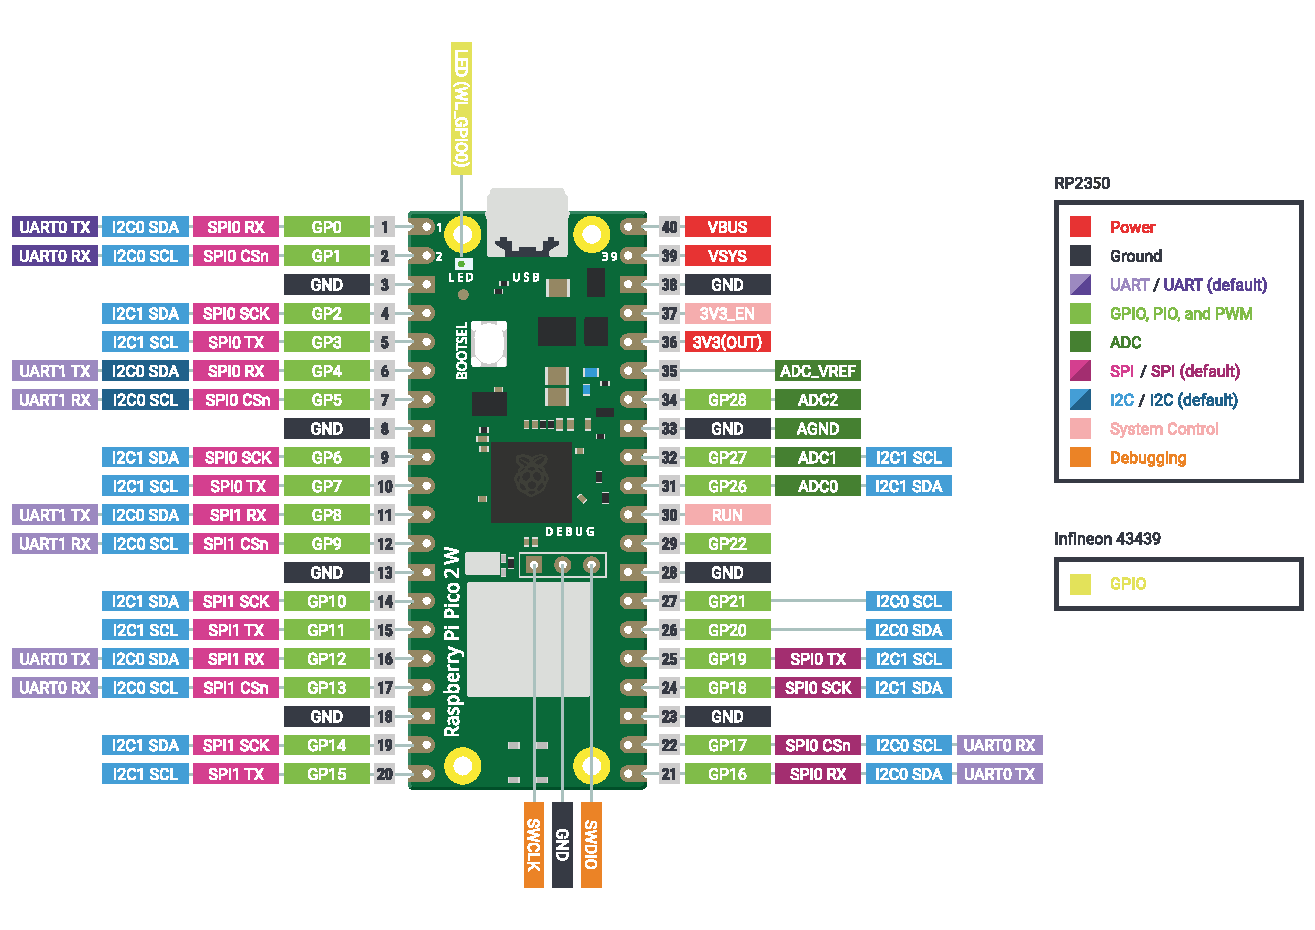
\includegraphics[width=0.90\textwidth]{files/Tobias/pics/Pinout/pico2w-pinout.pdf}
\caption[Raspberry Pico W - Pinout]{Raspberry Pico W - Pinout}
\label{fig:PicoW_Pinout}
\end{figure}




Um ein möglichst sauberes Design zu erreichen, wurde die Pin-Zuordnung des Mikrocontrollers folgendermaßen gewählt:

\renewcommand{\arraystretch}{1}

\begin{table}[H]
\centering
\rowcolors{2}{white}{white}
\begin{tabular}{|l|c|}
\hline
\rowcolor{cyan!20}
\textbf{GPIO-Pin} & \textbf{Funktion} \\
\hline
GPIO0 & S1 \\
\hline
GPIO1 & S2 \\
\hline
GPIO4 & SDA \\
\hline
GPIO5 & SCL \\
\hline
GPIO6 & Busy \\
\hline
GPIO7 & RST \\
\hline
GPIO8 & DC \\
\hline
GPIO9 & CS \\
\hline
GPIO10 & CLK \\
\hline
GPIO11 & DIN (MOSI) \\
\hline
\end{tabular}
\caption{GPIO-Zuordnung des Raspberry Pico W}
\label{tab:GPIO_Zuordnung}
\end{table}


In Tabelle \ref{tab:GPIO_Zuordnung} sind GPIO0 und GPIO1 dem Auslesen der Taster S1 und S2 (Kap. \ref{sec:Benutzer_Interaktionen}) zugewiesen. GPIO4 und GPIO5 sind den I2C-Kommunikationsleitungen zugeordnet; auf diesen Pins liegt das „Default-I2C“ des Raspberry Pi Pico W (Abb. \ref{fig:PicoW_Pinout}). GPIO7 bis GPIO11 dienen zur Ansteuerung des Displays mit SPI (Abb. \ref{fig:Display_Pinout}).

\bigskip \\

\textbf{Display - Pinout:}

\begin{figure}[!htb]
\centering
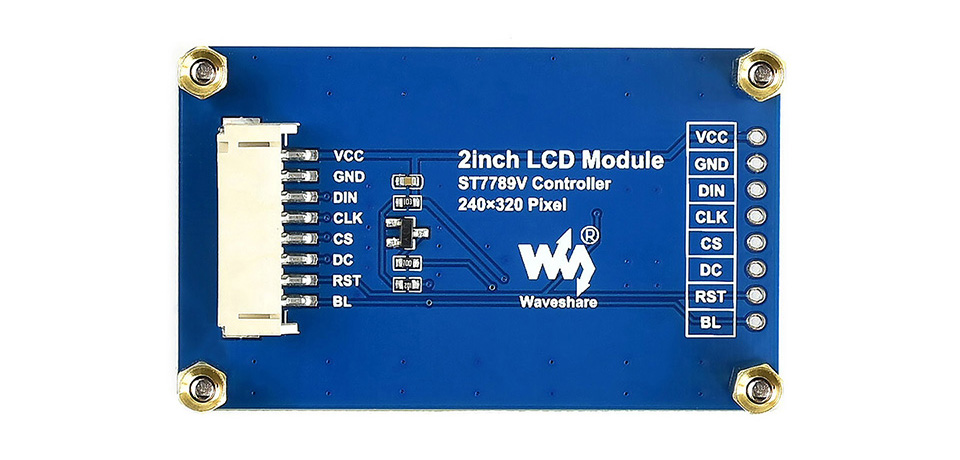
\includegraphics[width=0.7\textwidth]{files/Tobias/pics/Pinout/2inch-LCD-Module-4_960.jpg}
\caption[Display - Pinout]{Display - Pinout}
\label{fig:Display_Pinout}
\end{figure}


\begin{table}[H]
\centering
\begin{tabular}{|l|l|}
\hline
\rowcolor{cyan!20}
\textbf{Pin} & \textbf{Funktion} \\
\hline
VCC & Versorgung (3{,}3V / 5V) \\
\hline
GND & Ground \\
\hline
DIN & SPI-Dateninput \\
\hline
CLK & SPI-Taktinput \\
\hline
CS & Chip-Select, Low-Active \\
\hline
DC & Daten-/Befehlauswahl (High = Daten, Low = Befehl) \\
\hline
RST & Reset, Low-Active \\
\hline
BL & Hintergrundbeleuchtung \\
\hline
\end{tabular}
\caption{Pinbelegung des Displays}
\label{tab:display_pins}
\end{table}

\bigskip \\

\textbf{PASCO2 - Pinout:}

\begin{figure}[!htb]
\centering
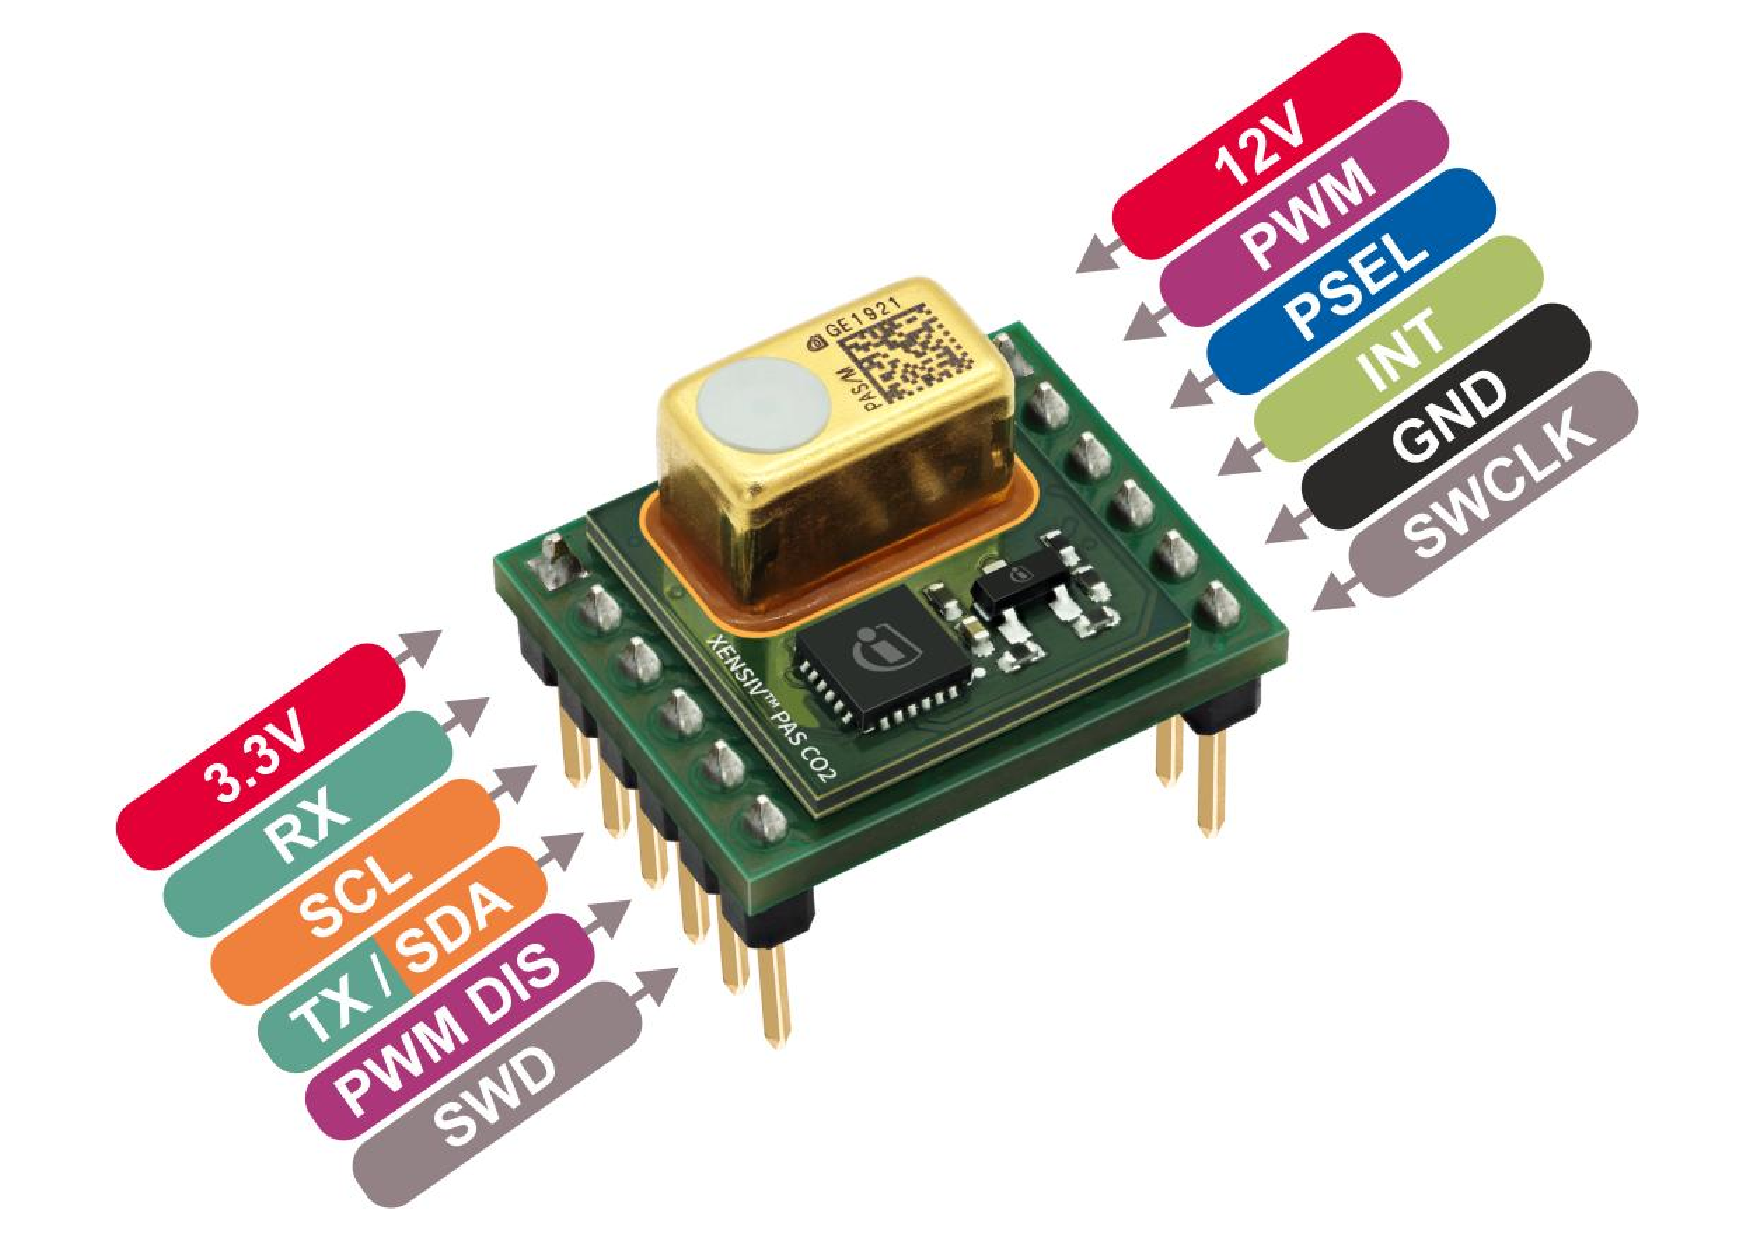
\includegraphics[width=0.6\textwidth]{files/Tobias/pics/Pinout/minieval_co2_pinout.pdf}
\caption[Display - Pinout]{Display - Pinout}
\label{fig:PASCO2_Pinout}
\end{figure}

Mithilfe des PSEL-Pins wird dem Sensor mitgeteilt, welche Kommunikationsschnittstelle verwendet wird. In diesem Fall wird PSEL für I2C auf GND gezogen.

\bigskip \\

\textbf{BME688 - Pinout:}

\begin{figure}[!htb]
\centering
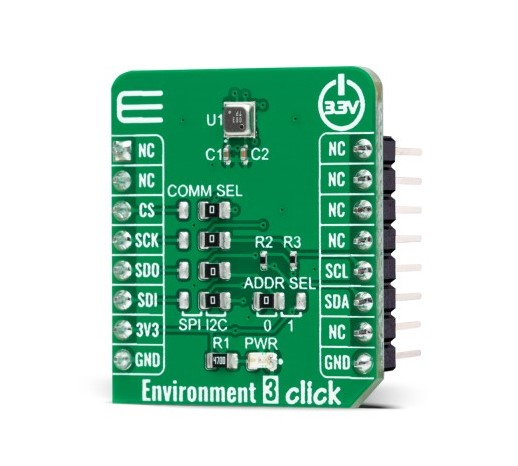
\includegraphics[width=0.5\textwidth]{files/Tobias/pics/Pinout/environment-3-click-thickbox_default-2.jpg}
\caption[Display - Pinout]{Display - Pinout}
\label{fig:BME688_Pinout}
\end{figure}

Wie in Abbildung \ref{fig:BME688_Pinout} zu sehen ist, befinden sich verschiedene Auswahlmöglichkeiten auf dem ...Board, die mithilfe von Lötbrücken genutzt werden können. Die Kommunikationsschnittstelle kann zwischen SPI und I2C gewählt werden (in diesem Fall I2C), ebenso wie die Adresse des Sensors (0 = 0x76, 1 = 0x77). 





      \section{USB-C}

      Das Messgerät benutzt USB-C für die Spannungsversorgung. Da nur die Versorgungsleitungen des USB-Busses benutzt werden, wird eine USB4125-Buchse verwendet (Kap. \ref{sec:USB4125_75}). Diese hat nur die Versorgungs-, GND- und CC-Pins, welche ausreichend sind, da keine Daten übertragen werden müssen. Ebenfalls erleichtert diese Buchse das Auflöten auf die Platine.

\begin{figure}[!htb]
\centering
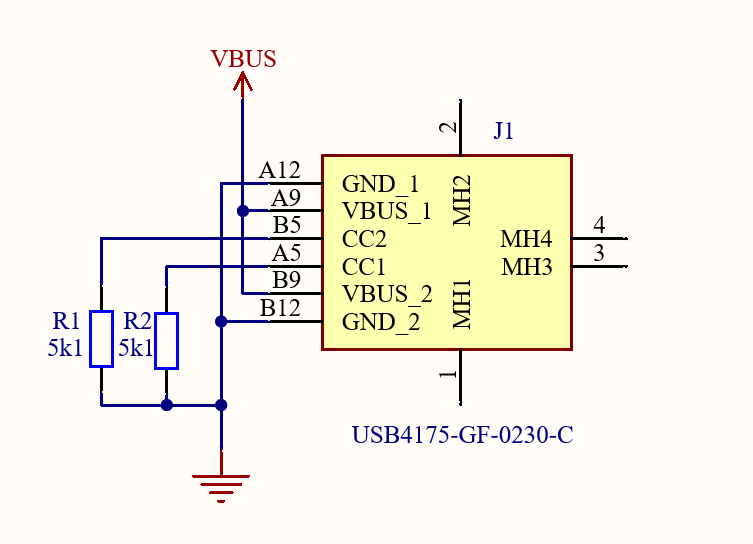
\includegraphics[width=0.75\textwidth]{files/Tobias/pics/Schaltungen/Schematik/USBC_Schematik.PNG}
\caption[USB-C Schematik]{USB-C Schematik}
\label{fig:USB-C_Schematik}
\end{figure}

Wie in Abbildung \ref{fig:USB-C_Schematik} zu sehen ist, sind beide CC-Pins der USB-C-Buchse über 5,1-k$\Omega$ Widerstände mit GND verbunden. Bei USB-C erfolgt über diese Pins der Austausch über die Verbindungskonfigurationen. Die 5,1-k$\Omega$ Widerstände signalisieren, dass es sich bei dem angeschlossenen Gerät um einen Verbraucher handelt, der maximal 15W Leistung aufnehmen darf \cite{USBCPowerDelivery}.

\begin{figure}[H] 
  \centering

  \begin{subfigure}[b]{0.48\textwidth}
    \centering
    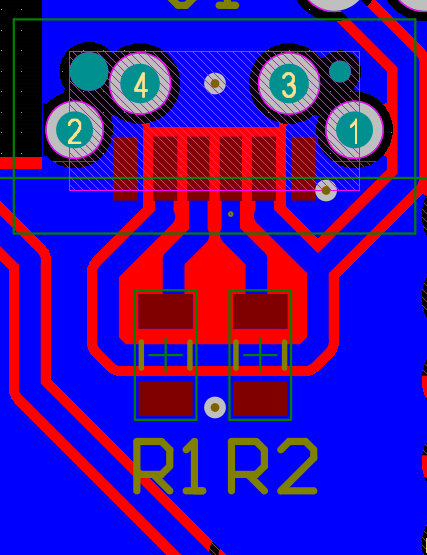
\includegraphics[height=7cm]{files/Tobias/pics/Schaltungen/PCB/USB_C_PCB.PNG}
    \caption{USB-C Bottom Layer}
    \label{fig:USB-C_Bottom_layer}
  \end{subfigure}
  \hfill
  \begin{subfigure}[b]{0.48\textwidth}
    \centering
    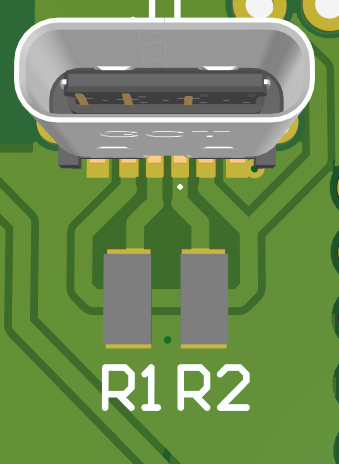
\includegraphics[height=7cm]{files/Tobias/pics/Schaltungen/PCB/USB_C_PCB_3D.PNG}
    \caption{USB-C 3D Ansicht}
    \label{fig:USB-C_3D_Ansicht}
  \end{subfigure}

  \caption{USB-C PCB Ansicht}
  \label{fig:pcb_layers}
\end{figure}



      \section{3,3V Spannungsregler}

Da der Mikrocontroller, die Sensoren sowie das Display mit 3,3V arbeiten und die USB-C-Versorgung 5V bereitstellt, ist ein Spannungsregler notwendig. Verwendet wird der NJM12856 \cite{NJM12856}, da dieser mit 1000mA dem maximalen Strom des Geräts standhält (Tab. \ref{tab:Stromverbrauch}).

Um den maximalen Stromverbrauch des Gerätes zu bestimmen, wurden folgende Werte aus den Datenblättern der einzelnen Komponenten \cite{Raspberry_Pi_Pico_W}, \cite{PASCO2V01}, \cite{BME688}, \cite{LCDDisplayDatasheet} entnommen: 


\renewcommand{\arraystretch}{1}

\begin{table}[H]
\centering
\rowcolors{2}{white}{white}
\begin{tabular}{|l|c|}
\hline
\rowcolor{cyan!20}
\textbf{Komponente} & \textbf{max. Stromaufnahme} \\
\hline
BME688 & 18\,mA \\
\hline
PAS CO\textsubscript{2} & 160\,mA \\
\hline
Display & 45\,mA \\
\hline
Raspberry Pi Pico W & 300\,mA \\
\hline
\end{tabular}
\caption{max. Stromverbrauch der Hauptkomponenten}
\label{tab:Stromverbrauch}
\end{table}

Da für den Raspberry Pico W keine genaue Angabe über den Stromverbrauch im Datenblatt zu finden ist, wurde der obige Wert durch Internetrecherche \cite{PicoWCurrent} und unter Einbezug der benutzten Bussysteme sowie der WLAN-Verbindung geschätzt.

\begin{figure}[!htb]
\centering
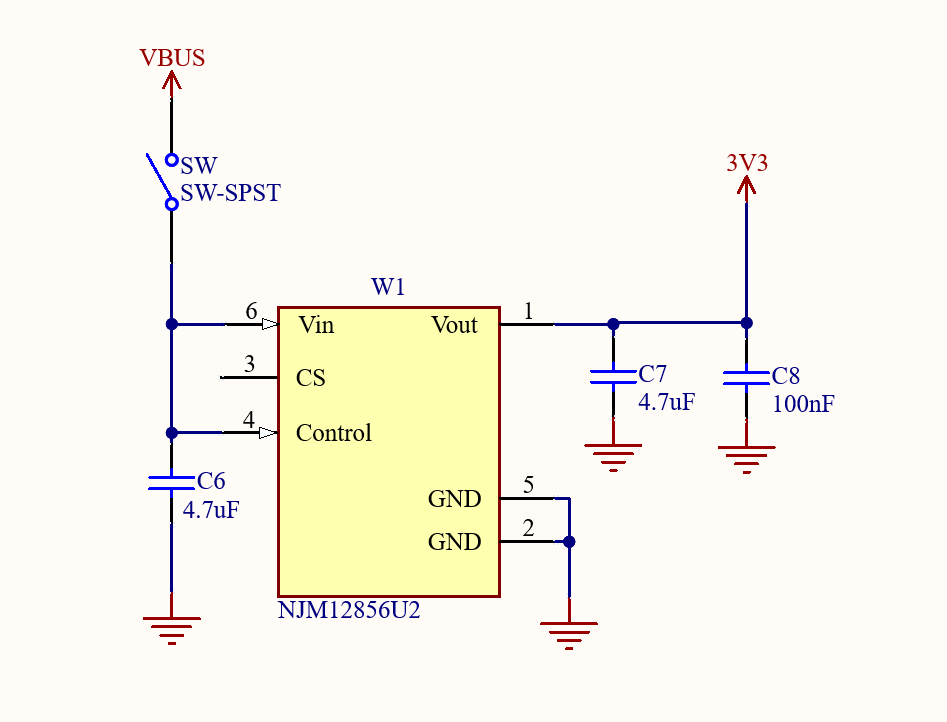
\includegraphics[width=0.75\textwidth]{files/Tobias/pics/Schaltungen/Schematik/3V3_Converter_Schematik.PNG}
\caption[3,3V Spannungsregler Schematik]{3,3V Spannungsregler Schematik}
\label{fig:3,3V Spannungsregler Schematik}
\end{figure}

Wie in Abbildung \ref{fig:3,3V Spannungsregler Schematik} zu sehen ist, wurde am Ein- und Ausgang des NJM12856 jeweils ein 4,7µF-Kondensator hinzugefügt, um stabile Spannungen zu gewährleisten. Zusätzlich wurde ein weiterer 100nF-Kondensator am Ausgang des NJM12856 hinzugefügt, um mögliche Störungen zu minimieren. Der CS-Pin bleibt offen, da kein Softstart benötigt wird \cite{NJM12856}. 2 Pins wurden für einen Schalter inkludiert, um die gesamte Spannungsversorgung vom Gerät zu trennen. 


\begin{figure}[H] 
  \centering

  \begin{subfigure}[b]{0.48\textwidth}
    \centering
    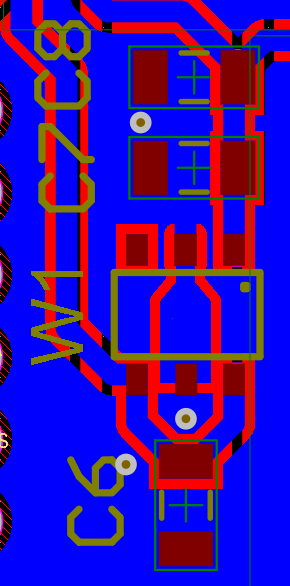
\includegraphics[height=7cm]{files/Tobias/pics/Schaltungen/PCB/3V3_Spannungregler_PCB.PNG}
    \caption{3,3V Spannungsregler Bottom Layer}
    \label{fig:USB-C_Bottom_layer}
  \end{subfigure}
  \hspace{2mm} % <-- Abstand verkleinert
  \begin{subfigure}[b]{0.48\textwidth}
    \centering
    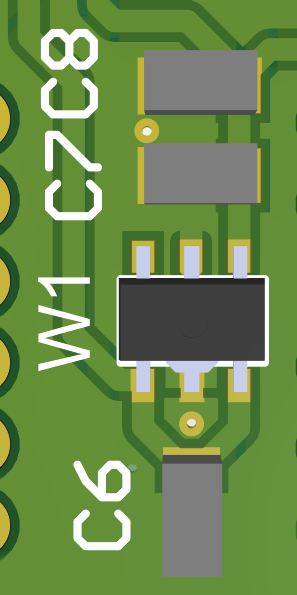
\includegraphics[height=7cm]{files/Tobias/pics/Schaltungen/PCB/3V3_Spannungsregler_PCB_3D.PNG}
    \caption{3,3V Spannungsregler 3D Ansicht}
    \label{fig:USB-C_3D_Ansicht}
  \end{subfigure}

  \caption{3,3V Spannungsregler PCB Ansicht}
  \label{fig:pcb_layers}
\end{figure}








      \section{12V Spannungwandler}
      
Der PASCO2V01-Sensor benötigt neben der 3,3V-Spannungsversorgung ebenfalls eine 12V-Spannungsversorgung. Der Aufwärtswandler TLV61046ADBVR \cite{TLV61046} wird dafür benutzt. Dieser ist in dem Datenblatt für Design-Richtlinien des PASCO2V01 \cite{PASCO2_Design_Guidelines}, inklusive Beschaltung, empfohlen.


\begin{figure}[!htb]
\centering
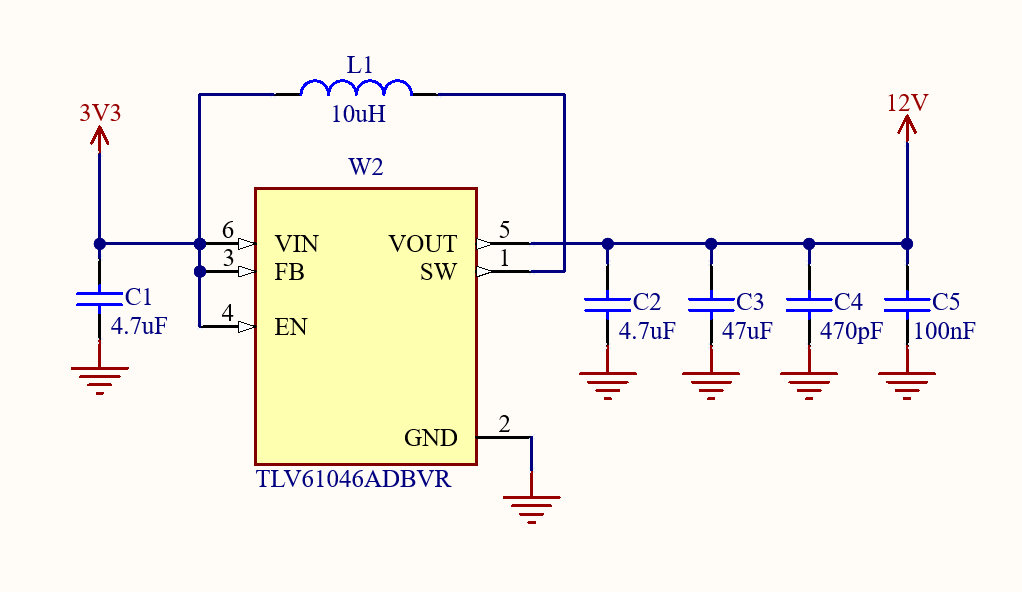
\includegraphics[width=0.75\textwidth]{files/Tobias/pics/Schaltungen/Schematik/12V_Converter_Schematik.PNG}
\caption[12V Spannungswandler Schematik]{12V Spannungswandler Schematik}
\label{fig:12V Spannungswandler Schematik}
\end{figure}

Die Beschaltung des TLV61046ADBVR (Abb. \ref{fig:12V Spannungswandler Schematik}) wurde entsprechend dem Datenblatt für Design-Richtlinien des PASCO2V01 \cite{PASCO2_Design_Guidelines} entnommen. 


\begin{figure}[H] 
  \centering

  \begin{subfigure}[b]{0.48\textwidth}
    \centering
    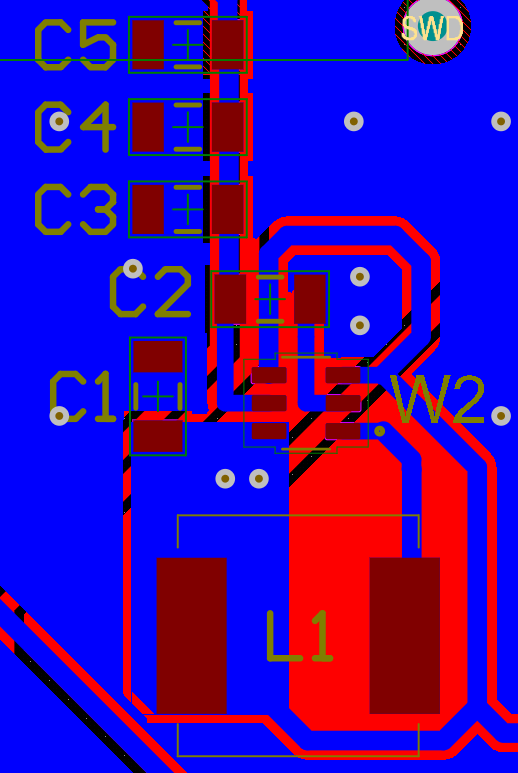
\includegraphics[height=7cm]{files/Tobias/pics/Schaltungen/PCB/12V_Spannungswandler_PCB_.PNG}
    \caption{12V Spannungswandler Bottom Layer}
    \label{fig:12V_Bottom_layer}
  \end{subfigure}
  \hfill
  \begin{subfigure}[b]{0.48\textwidth}
    \centering
    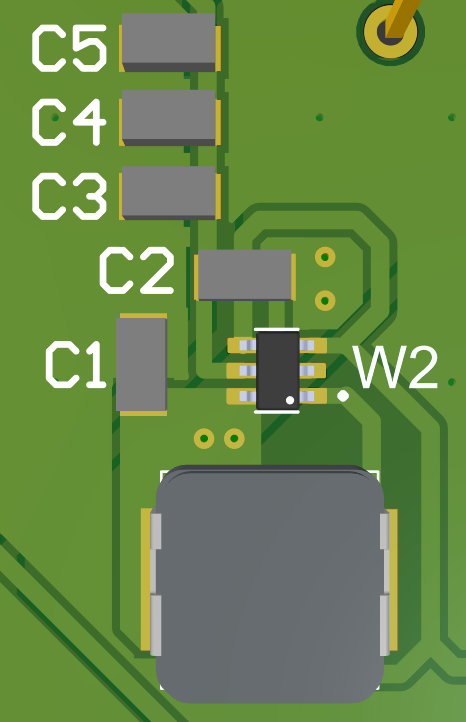
\includegraphics[height=7cm]{files/Tobias/pics/Schaltungen/PCB/12V_Spannungswandler_PCB_3D.PNG}
    \caption{12V Spannungswandler 3D Ansicht}
    \label{fig:12V_3D_Ansicht}
  \end{subfigure}

  \caption{12V Spannungswandler PCB Ansicht}
  \label{fig:pcb_layers}
\end{figure}
      


   \section{PCB Version 1}
   \label{ref:PCB_Version_1}


   \begin{figure}[H] 
  \centering
  \begin{subfigure}[b]{0.48\textwidth}
    \centering
    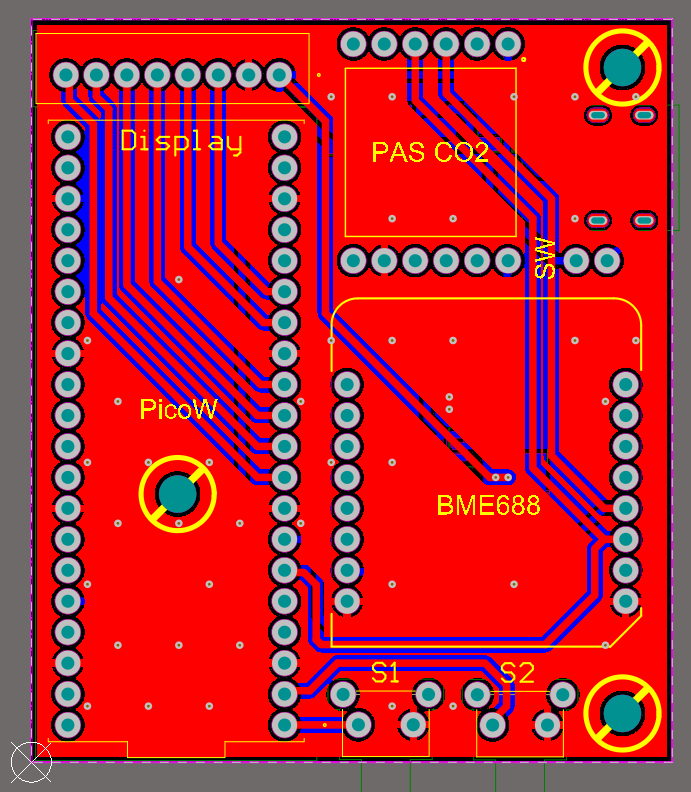
\includegraphics[height=7cm]{files/Tobias/pics/Schaltungen/PCB/Version1_Top.PNG}
    \caption{PCB Version 1 - Top Layer}
    \label{fig:PCB_Version1_Top}
  \end{subfigure}
  \hfill
  \begin{subfigure}[b]{0.48\textwidth}
    \centering
    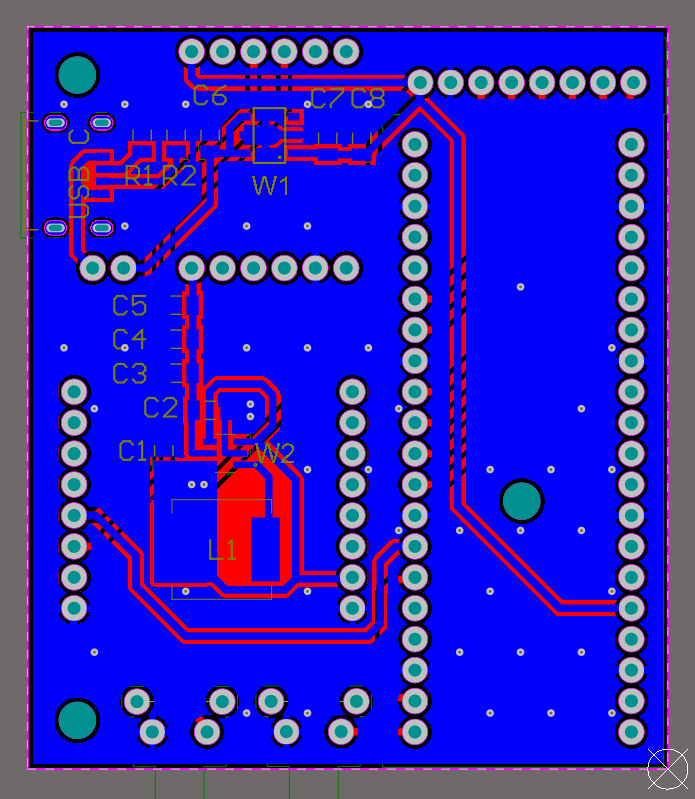
\includegraphics[height=7cm]{files/Tobias/pics/Schaltungen/PCB/Version1_Bottom.PNG}
    \caption{PCB Version 1 - Bottom Layer}
    \label{fig:PCB_Version1_Bot}
  \end{subfigure}
  \caption{PCB Version 1}
  \label{fig:PCB_Version_1}
\end{figure}

Da das Display im Gehäuse befestigt wird und sich nicht direkt auf der Platine befindet, wurde ein JST XH 2.54mm-Stecker (Female) für dessen Verbindung benutzt. Als Taster wurden 2-1825027-0 Taster verwendet. Diese sind geknickt und haben eine Knopflänge von 9,24mm. Dadurch lassen sich die Taster gut in das Gehäuse integrieren. Für die Befestigung im Gehäuse wurden auf der Platine 2 Löcher für M3-Schrauben vorgesehen. Ein drittes Loch direkt unter dem Mikrocontroller dient nur als Platzhalter.

  
\section{PCB Version 2}


   \begin{figure}[H] 
  \centering
  \begin{subfigure}[b]{0.48\textwidth}
    \centering
    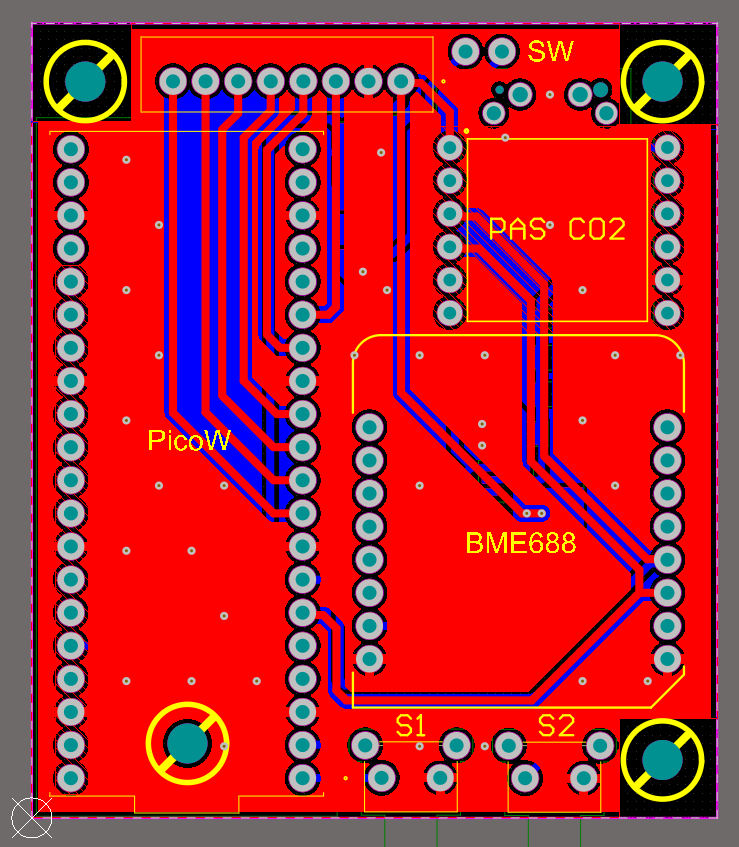
\includegraphics[height=7cm]{files/Tobias/pics/Schaltungen/PCB/Version2_Top.PNG}
    \caption{PCB Version 2 - Top Layer}
    \label{fig:PCB_Version2_Top}
  \end{subfigure}
  \hfill
  \begin{subfigure}[b]{0.48\textwidth}
    \centering
    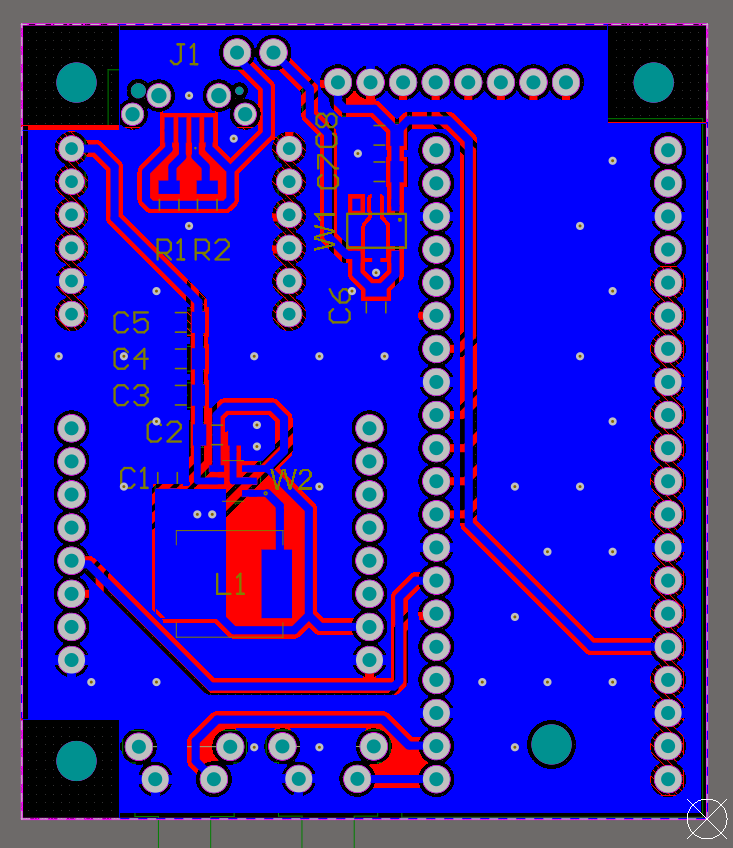
\includegraphics[height=7cm]{files/Tobias/pics/Schaltungen/PCB/Version2_Bottom.PNG}
    \caption{PCB Version 2 - Bottom Layer}
    \label{fig:PCB_Version2_Bot}
  \end{subfigure}
  \caption{PCB Version 2}
  \label{fig:PCB_Version_2}
\end{figure}

Für eine bessere Benutzerfreundlichkeit wurde die USB-C-Buchse von der ursprünglich seitlichen Position auf die Rückseite des PCBs gesetzt. Ebenfalls vereinfacht dies die Integration in das Gehäuse. Dabei wurde von einer USB4125-Buchse auf eine USB4175-Buchse (Kap. \ref{sec:USB4125_75}) gewechselt. Zusätzlich wurde ein weiteres Loch für eine Schraube zur Befestigung im Gehäuse eingebaut. Die ursprünglichen Positionen der SMD-Bauteile sowie der Sensoren wurden ebenfalls geändert.

   \begin{figure}[H] 
  \centering
  \begin{subfigure}[b]{0.48\textwidth}
    \centering
    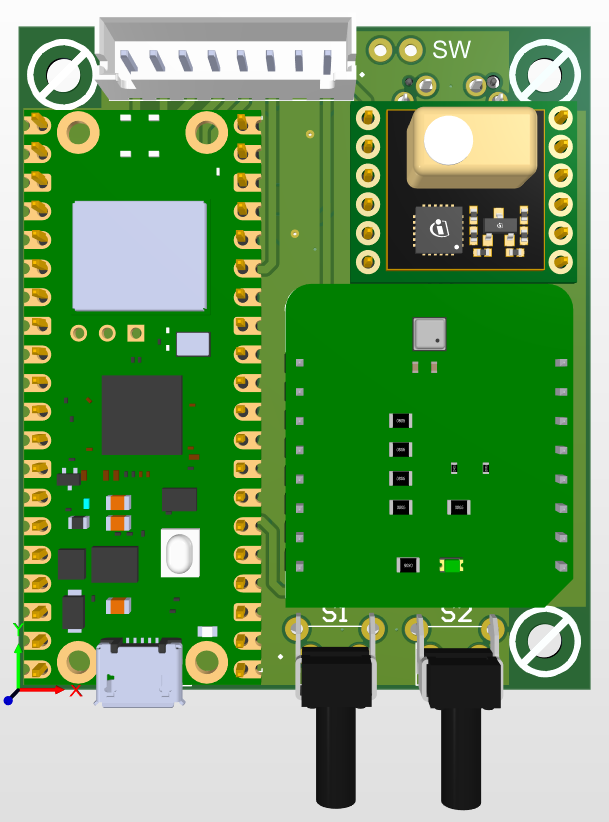
\includegraphics[height=7cm]{files/Tobias/pics/Schaltungen/3D/Top_Layer_3D.PNG}
    \caption{PCB Version 2 - Top Layer 3D Ansicht}
    \label{fig:PCB_Version2_Top_3D}
  \end{subfigure}
  \hfill
  \begin{subfigure}[b]{0.48\textwidth}
    \centering
    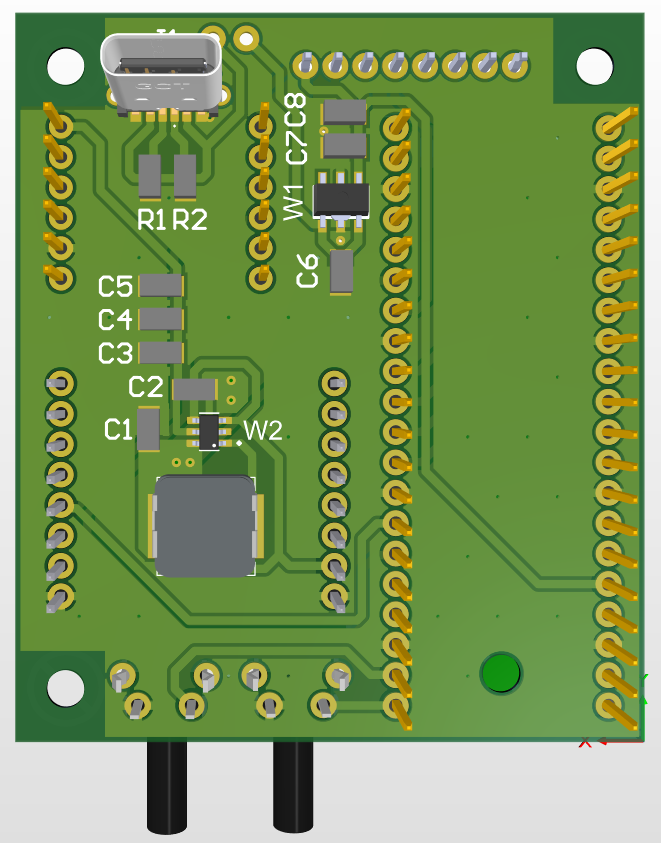
\includegraphics[height=7cm]{files/Tobias/pics/Schaltungen/3D/Bottom_Layer_3D.PNG}
    \caption{PCB Version 2 - Bottom Layer 3D Ansicht}
    \label{fig:PCB_Version2_Bot_3D}
  \end{subfigure}
  \caption{PCB Version 2 - 3D Ansicht}
  \label{fig:PCB_Version_2_3D}
\end{figure}



\section{Fertigung des PCBs/Prints}

Die zweite PCB-Version wurde bei JCL PCB bestellt und im Anschluss eigenständig bestückt. Da der mitgelieferte Verbindungstecker das Displays sehr lange Kabel hat und diese im Gehäuse zu viel Platz verbrauchen würden, wurden diese von 18cm Länge auf 10cm gekürtzt. Am abgetrennten Ende wurde ein JST XH 2.54mm-Stecker (Male) befestigt.



\section{Messungen}
	\subsection{Spannungen}

    Nach der Bestückung der Platine wurden die Versorgungsspannungen mit einem Multimeter überprüft. Sowohl die 3,3V- als auch die 12V-Versorgung waren mit minimalen Abweichungen korrekt.

\end{inhalt}